\subsection{\name{'s} transition patterns}
\label{sec:transition-patterns}

We first highlight six workflow patterns that are supported in most workflow
systems and also expressible in \name{}. Developers commonly use all or a
subset of these patterns to compose complex serverless workflows. We describe
each pattern and a set of real serverless applications that are built with one
or a combination of multiple patterns.

% We have identified six workflow transition patterns as the main building
% blocks to build arbitrary workflow compositions. These patterns are simple to
% use and yet expressive. These patterns include: \shadi{should we add sentence
% on how fold and for are unique?}

% \squishlist
\begin{itemize}
    \item \textit{\textbf{chain:} }
    Chaining is a simple but fundamental orchestration pattern. For example,
    an application might include a function (the source) that processes input
    data from a sensor followed by another function (the target) that adjusts
    an actuator based on the processed input. The \texttt{chain} pattern
    connects the two functions by invoking the target function with the source
    function's result.

    \item \textit{\textbf{fan out:}} 
    Another common pattern processes the output of a function in different
    ways in parallel. For example, an social network application might perform
    several independent functions given a new user post, such as URL
    shortening and resolving other users mentioned in the post. The
    \texttt{fan-out} pattern launches a vector of functions (branches) each
    with the output of the same source function.

	\item \textit{\textbf{map: }}
    An application may also perform the same function on multiple outputs of a
    source function. For example, a photo management application might unpack an
    archive of high-resolution images in one function and perform compression on
    each of the resulting images. The \texttt{map} pattern invokes the same
    function once for each element in a vector of outputs from the source
    function.

	\item \textit{\textbf{fan in:}}
    After processing data with many parallel branches, applications commonly
    want to aggregate results. For example, to build an index of a large
    corpus, the application might process a chunks in parallel and the
    aggregate the results. \texttt{fan-in} is a common pattern to join back
    multiple parallel functions, by invokeing a single ``sink'' function with
    the outputs from a vector of functions (the fan-in branches).

    \item \textit{\textbf{branch:}}
    An application may decide to take a different branch of the workflow graph
    based on runtime behavior (e.g., the output of a function). For instance,
    an ML application might use a function to first characterize the data and
    then select a model based on the features. The \texttt{branch} pattern
    selects a next function based on some boolean condition.

	\item \textit{\textbf{fold:}}
    \texttt{fold} sequentially applies the same function on the outputs of
    a vector of source functions, while aggregating with the intermediate
    results of running the function so far. For example, a video encoding
    application might encode chunks in parallel and then concatenate the
    results in order: concatenating chunk 1 and 2, then concatenating
    chunk 3 to chunk [1--2], and so on. \texttt{fold} is an advanced
    pattern that is not supported by all existing systems (e.g., AWS Step
    Functions do not support \texttt{fold}) but is expressible in \name{}.
% \squishend
\end{itemize}

% \vspace{-1ex}


Developers have built a variety of serverless workflows using these patterns,
ranging from simple 2-function chains to complex 1000s-of-functions
applications that aggregate large amounts of data from parallel pipelines.
Below we describe how four representative real-world applications, taken from
serverless application repositories and prior research, and them map to these
patterns.



\noindent\underline{\textit{IoT Pipeline:}} A HVAC control application (in
AWS serverless repository~\cite{iot-pipeline}) consisting of two functions
connected with a simple chain pattern: a function that aggregates
time-series data on indoor climate readings, followed by a HVAC system
control function that adjusts the HVAC settings based on the aggregate
statistics.

\noindent \underline{\textit{Text Processing:}} A component of the
DeathStarBench~\cite{deathstar} social network application that processes
user posts. The workflow consists of 5 functions, following the overall
structure of Figure \ref{fig:arch:unum-compile-time}. It fans out to two
branches that resolves user mentions and shortens URLs in parallel.
Lastly, it fans in to a function that saves the post along with resolved
user mentions and shortened URLs in a NoSQL database.

 \noindent \underline{\textit{MapReduce wordcount:}} A word count
application (from MapReduce~\cite{mapreduce}) counting the number of each
word in a dataset. The workflow dynamically creates many mappers each
processing a subsection of a dataset and then a fixed number of reducers
the aggregates mapper outputs.

\noindent\underline{\textit{ExCamera:}} is a novel video encoder
~\cite{excamera} that encodes large raw videos with thousands of parallel
functions to achieve low latency. This application has a complex workflow with
use of multiple patterns, as shown in Figure~\ref{fig:excamera}. The workflow
consists of three stages. First, an ``encode'' stage that chunks the video and
runs multiple pipelines of encoding and decoding functions entirely in
parallel. Next, each branch $i$ combines results from the previous branch to
re-encode the video. This step involves a fan-ins between adjacent branches in
the previous stage. Finally, all encoded video chunks are concatenated into
the a single video stream using a fold pattern.


We implement all of the above applications with \name{} and evaluate their
costs and performance in \S\ref{sec:eval}. In the following section, we will
describe how we execute each pattern in a completely decentralized manner.

\begin{figure}[t!]
	\centering
	\scalebox{.9}{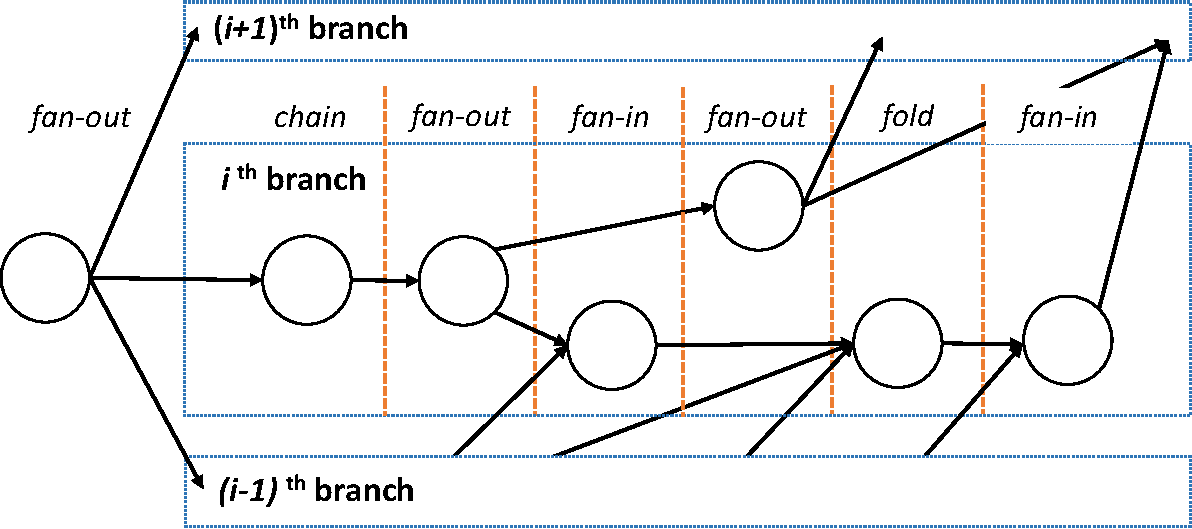
\includegraphics[width=\columnwidth]{figures/excamera.pdf}}
	\caption{ExCamera breakdown of workflow transition patterns. }
	\label{fig:excamera}
\end{figure}


%\name{} supports four general  control-flow/transition patterns: \shadi{do we want to use the name "transition" or "control-flow". Lets be consistent throughout.}
%\begin{itemize}
%	\item \textit{chain} ($f\rightarrow g$): where $g$ is invoked with the output of $f$. Chaining is a simple but most fundamental control-flow pattern, e.g.,  a function processing sensor data followed by another function adjusting an
%	actuator. 
%	\item \textit{map}($f[o_1, ..., o_n]\rightarrow g$): where $g$ is invoked on  \textit{multiple} outputs of $f$. Map is a simple interface to create parallelism but on an identical function, e.g.,  a photo management application performs the same "compression" function on
%	each of the images in a unzipped folder. 
%	\item \textit{fan out} ($f\rightarrow [g_1, ..., g_n]$): where and array of (identical or different) functions, $g_1$ to $g_n$ are invoked in parallel with the output of $f$. Fan-out is a common pattern to create parallel processing,  e.g.,  an social network application performing
%	several independent functions given a new user post, such as URL shortening
%	and resolving other users mentioned in the post. 
%	\item \textit{fan in} ($[f_1, ...f_n] \rightarrow g$): where the output of $n$ (identical or different) parallel functions are aggregated and then $g$ is invoked on the array of \textit{all} outputs. This is a common pattern to join back multiple parallel functions, e.g.,\shadi{??}. 
%\end{itemize}
%
%\name{} applications/workflows are built by using arbitrary composition of  these patterns, e.g., a serverless video encoder that divides a large
%video into chunks(\shadi{?}), encodes each chunk in parallel (map) and concatenates all back
%at the end (fan-in).
%These four patterns  can express a rich variety of workflows
%efficiently, including a superset of workflows expressible in AWS Step
%Functions and all workflows we encountered. In the next section we describe how we execute these pattern with no orchestrator involved.


%
%\subsection{Decentralized execution of transitions}
%\label{sec:transition-execution}
%
%A key challenge in decentralizing control-flow is determining where to store
%control-flow state and how to execute transitions, without a global view of the orchestrator. \name{} decentralized each pattern by logically partitioning the transition into a pair of nodes:  an \textit{egress node(s)} appended to the
%upstream function and a matching \textit{ingress node(s)} prepended to the immediate
%downstream function(s).  Every user function is invoked once with a
%single value by an ingress node and outputs its result to a single egress
%node.  Figure~\ref{fig:transition} demonstrates the ingress/egress nodes added for each pattern. Each ingress/egress node performs a specific logic on the incoming/outgoing data depending on the transition pattern,  as we will discuss further below.  We note that transition patterns only uses the basic serverless abstractions, universally supported by current platforms, and are platform agnostic.
%Specifically, they relies
%on an asynchronous invocation API for FaaS functions and a strongly consistent
%data store that supports conditional writes (for fan-in and exactly-once guarantees only). 
%
%%Logically, each pattern is designed as
%%a pair of nodes: an ingress node and an egress node. The egress node is appended to the
%%upstream function and the matching ingress node is prepended to the immediate
%%downstream function(s).
%%Every user function in
%%\name{} has exactly one input edge coming from an ingress node and one output
%%edge going to an egress node, i.e., the user function is invoked once with a
%%single value by an ingress node and outputs its result to a single egress
%%node. 
%
%%The \name{} backend compiler converts the IR representation of functions  to platform specific \name{} runtimes with pairs of ingress/egress nodes (Figure \shadi{??}). The runtime then, based on the transition patterns embeded in \name{} config file, executes the patterns accordingly in each egress/ingress point. In this section we describe what exact execution logic does each pattern map to at the ingress and egress points. We note that \name{} runtime only uses the basic serverless abstractions, universally supported by current platforms, and are platform agnostic.
%%Specifically, it relies
%%on an asynchronous invocation API for FaaS functions and a strongly consistent
%%data store that supports conditional writes (for fan-in and exactly-once guarantees only). 
%
%\begin{figure}[t!]
%	\centering
%	\scalebox{.7}{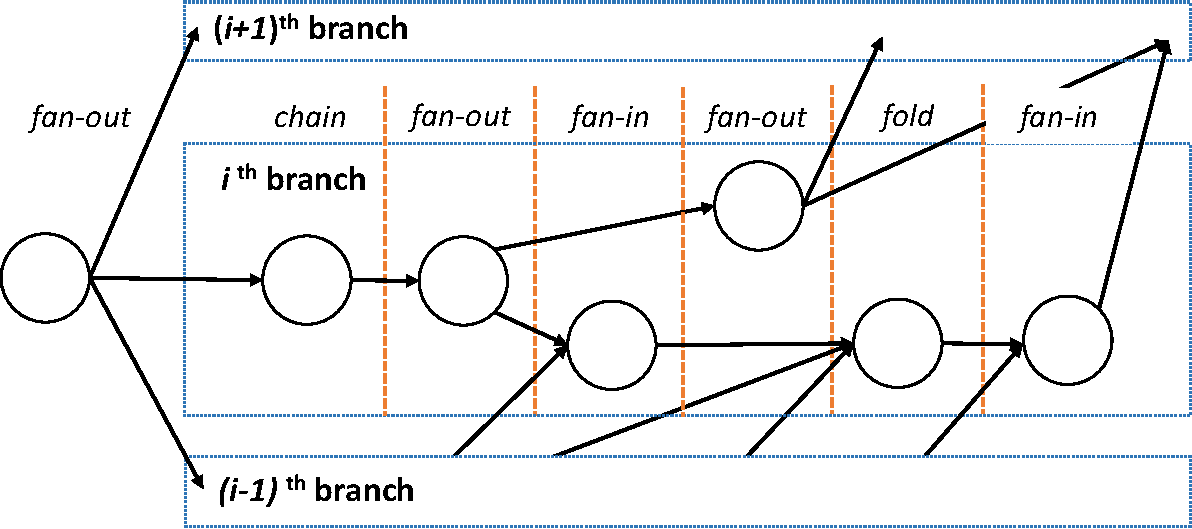
\includegraphics[width=\columnwidth]{figures/excamera.pdf}}
%	\caption{TODO}
%	\label{fig:excamera}
%\end{figure}
%
%\noindent\textbf{Chain:}
%The chain pattern invokes a single target function with the result of a source function.
%As shown in Figure~\ref{fig:transition}, chaining consists of one egress node 
%appended to the source function and one ingress is prepended to the target.
%At runtime, the egress node gets the output of the source user function
%and uses the platform's asynchronous function invocation API to call the
%target function directly from the source. The ingress on the target reads the
%data sent from source and passes it to the target user function. Depending on
%the platform's implementation of asynchronous invoke API, the ingress might
%read the input data from a data store or the received HTTP message.
%
%
%\noindent\textbf{Fan-out:}
%The fan-out processes the output of a function  in parallel, by 
%invoking vector of functions (branches) each with the output of the same
%source function. The fan-out pattern consists of one egress node and many ingress
%nodes (one per branch). Similar to chaining, the egress node runs with the
%source function and it uses the asynchronous invocation API to invoke each
%branch where each ingress node 
%reads the input data sent from the source and passes it to its user function.
%
%
%\noindent \textbf{Map:}
%The \texttt{map} gadget invokes the same
%function once for each element in a vector of outputs from the source
%function. The algorithm and placement of \texttt{map} ingress and egress nodes
%are identical to \texttt{fanOut}. \dhl{TODO: talk about the dynamic aspect of Map}
%\shadi{Map seems very empty. why do we have it separated? any details and challenges to add here? }
%
%
%
%
%\noindent\textbf{Fan-in:} The \texttt{fanIn} pattern takes the outputs from a vector of
%functions (the fan-in branches) and invokes a single ``sink'' function. As shown in Figure~\ref{fig:transition}, fan-in consists of one ingress prepended to the sink function and several egress nodes, each
%appended to a fan-in branch. Fan-in has an important requirement--the sink function should be called \textit{once} and only when \textit{all} fan-in branches have completed. At the same time, \name{} aims to avoid idle-billing and therefore extra billing (Section \shadi{??}). Thus, the fan-in pattern should be ``wait-free'' on both sides: a) the upstream functions should terminate after completion and not wait for each other, and b) the sink function should not  spin up ahead of time idly waiting for upstream functions to finish.
%
%% TBD
%%
%% The \texttt{fanIn} gadget gadget ensures that the control-flow transition is
%% \emph{wait-free} and that the sink function is invoked only once.
%% Specifically, its semantics is that the sink function is invoked only once
%% when all upstream functions in the vector have completed.
%
%% To realize the semantics, the \texttt{fanIn} gadget has to solve several
%% challenges. Access to branches data. wait-free. and synchronize.
%
%%The \texttt{fanIn} gadget ensures that the control-flow transition is
%%\emph{wait-free}. That is the sink function is invoked only when all upstream
%%functions in the vector have completed so that the sink function does have to
%%be spun up ahead of time and waste CPU cycles (and therefore extra billing)
%%idly waiting for upstream functions to finish. Moreover, the upstream
%%functions in \texttt{fanIn} simply terminates when done and do not wait for
%%each other either.
%
%To achieve this, \name{} uses an intermediary data store (as shown in Figure \shadi{??}) to log the output of upstream functions and signal the completion to the sink. In this design, each egress  node simply
%writes its output and terminates the function (avoiding idle-billing on the upstream functions), with the exception of the ``last'' egress node which first invokes the sink function. \name{} synchronizes among the upstream functions to identify the ``last'' function using an
%atomic read-after-write over a single object. Every upstream function \shadi{....? give a high-level idea. what is the process here, a few senteces in the data-store independent manner!}.  This ensures when the sink function is
%invoked, it is invoked only once.  Specific implementation depends
%on the data store as we discuss the details in \S\ref{sec:impl}.  Given that the data store is shared among all upstream functions, any egress node can see if another egress node has completed and any egress can invoke the sink function. 
%
%The ``last'' egress invokes the sink function with a vector of pointers
%to each upstream function's stored output. The pointers are the in same order
%as the vector of upstream function names.\shadi{does this point regarding the naming matter? if so, add some details. If not, maybe remove?} The ingress on the sink function
%dereferences each point by reading from the data store and passes a vector of
%output values to its user function.
%
%
%We have implemented \name{} with both Dynamo DB and S3. However, \name{} can be integrated with any data-store as long is it provides strong consistency with conditional writes. Strongly consistent is required to prevent the
%scenarios where all egress nodes have written outputs but none of them sees that all
%have completed, which will result in the sink function never being invoked. \shadi{wouldn't eventual be enough? the sink will eventually be invoked}
%\shadi{give insight why you need conditional writes. this comes out of the blue}. 
%\dhl{?TODO: Say more about synchronization? That it needs to be idempotent
%	because functions can crash and be retried.}
%
%
%%To achieve this, the \texttt{fanIn} egress always writes the output of its
%%user function to a data store. This serves two purposes: (1). it allows any of
%%the upstream functions to access the output of other upstream functions (2).
%%it signals the completion of a function. This way, each egress can simply
%%writes its output and terminate. 
%%
%%Other egress nodes can still access completed
%%egress' data after they terminate. Any one of the egress can invoke the sink
%%function. And any one of the egress can see if other egress has completed or
%%not. \dhl{definitely needs better phrasing but hopeful the point makes sense}
%
%
%
%
%
%
%\dhl{?TODO: Fan-in is a critical control-flow pattern to support and distinguishes \name{}
%	from ad-hoc trigger-based composition.  Do we want to constrast here? and what
%	should we say? Different from ad-hoc compositions: 1. use of data store 2.
%	Control flow logic not only on the caller but also on the callee 3. standard,
%	off-the-shelf primitives that's not application specific that developers build
%	from scratch.}
%
%\dhl{?TODO: Fan-in expresses data dependencies. More flexible/expressive than
%	Step Functions because SF only supports dependencies within a state. unum
%	fan-in can specify any function in the workflow.}
%
%
%
%
%
%
%
%
%
%
%
%
%
%\shadi{:::::::::left over comments. not sure if they need to be addressed?}
%
%
%
%%
%%\amit{TODO: I feel like there is a bunch of complexity, particularly with
%%	fan-in, do with assigning indexes to branches, etc, that is part of the
%%	platform-agnostic design of unum, so should be here. But I don't recall the
%%	specifics. Are there also similar things for the other gadgets?}
%%\dhl{I'm not sure what you mean by "similar things". But the branch indexes
%%	are assigned by the fan-\emph{out} node. The purpose is to give each node in
%%	the graph a unique name. I really don't think we should discuss the naming
%%	aspect in this section. I think this structure of writing the design works
%%	very well if we keep the gadgets to be general algorithms for control-flow
%%	patterns that are designed against an abstract serverless machine. We can talk
%%	about what we require from the serverless abstraction, but we shouldn't talk
%%	about the naming scheme. The gadget just cares that each function has a name,
%%	that you can identify them. It does not care how. Then in the IR section, we
%%	can talk about how the IR actually encodes the gadgets, and that's where we
%%	can explain that (1). we need each function to have a unique name for fan-in
%%	to work because we need to clearly identify which node's result to fan-in
%%	from, and we can have multiple instances of the same function in the graph
%%	because of fan-in and map. (2). our naming scheme is to assign an integer,
%%	starting with 0 and incrementing monotonically by 1, to each branch. And
%%	that's it. That's all the information we need at the IR level. And finally in
%%	the runtime section, we show the input payload which has a field for the
%%	branch index, and that's how we actually implement this piece of information.
%%	And we explain that the fan-out node adds this field to the payload when
%%	invoking each branch. It's like the storage layers where each layer adds a bit
%%	more information to enable specific additional functionalities.}
%
%
%
%
%% chain = invoke, fan-out = a bunch of invoke, one for each continuation;
%% Additionally, in the case of Map, one invoke for each element of the array
%% (output of the user function).  fan-in .... well.... let's see. The semantics
%% is: invoke the fan-in function once when all of its inputs are ready. In
%% practice, it is each branch synchronize over the data store to see if all
%% branches have completed. The last branch to complete calls invoke on the fan-in
%% function, and pass it pointers to all branches results/checkpoints in the data
%% store. The fan-in function first reads the branches' results, in order, via the
%% pointers, then pass them as input to the user code.
%
%\dhl{"strongly consistent data store with conditional writes". Is this going
%	to raise eyebrows when we later mention S3? Because technically, S3 does not
%	have a conditional write API. We implement it with its object versions
%	feature, which has to be turned on when creating the bucket. Maybe better to
%	call it something else.}
%
%% \dhl{I'm not sure it makes sense to treate fan-in specially on the directed
%	% graph level. In the previous version, the ingress gadget node on the fan-in
%	% doesn't really perform any \emph{control-flow logic}. It just reads the input
%	% data. And this is the same behavior across all gadgets. The ingress just read
%	% data, whether from a HTTP packet or from DynamoDB. You can pass a vector of
%	% pointers via a chain gadget and the ingress will do the same thing. But I
%	% guess more importantly, the ingress is simply and uniform enough that treating
%	% fan-in specially in our explanation doesn't add much value.}
%
%\dhl{From previous version: "At compile-time, \name{} injects these gadgets
%	into the nearest function and executes them in the \name{} runtime that wraps
%	the function. Thus there is no system overhead for running the gadgets---they
%	are, effectively, embedded in the functions themselves."The last sentence is
%	unclear to me. Running gadgets incur latency and additional Lambda billing.}
%
%%%%%%%%%%%%%%%%%%%